\documentclass[]{article}
\usepackage{amsfonts}
\usepackage{amsmath}
\usepackage{graphicx}
\usepackage{hyperref}
%opening
\title{A case study of the 2019-2020 Lombardy COVID-19 outbreak using a SIR Model.}
\author{Umberto Zerbinati}

\begin{document}

\maketitle

\begin{abstract}

\end{abstract}

\section{SIR Model}
The SIR model is a system of ODEs design to model the dynamics of an epidemics not affected by birth and death. This model was originally developed by Kermack-McKendrick in 1927, and is expressed by the following ordinary differential equations:
\begin{align}
	\label{eq:SIR}
	\begin{split}
		S'(t) = -\beta S(t) \frac{I(t)}{N}\qquad N = S+I+R,\\
		I'(t) = \beta S(t) \frac{I(t)}{N}-\gamma I(t) \qquad S(0) = S_0,\\
		R'(t) = \gamma I(t)\qquad I(0)=I_0,\, R(0)=0.
	\end{split}
\end{align}
In particular $\beta$ is defined as the product between the average number of contacts per person times the probability the disease transmit at each contact, and $\frac{1}{\gamma}$ is the duration of the infection in days. An other important quantity is the average number of secondary infection, i.e. $R_0$, in particular in SIR model it is defined as $R_0 = \frac{\beta}{\gamma}$. This is known to be a some sort of magic number when it comes to epidemic spread. If we define the two quantity:
\begin{equation}
	x(t) = \frac{S(t)}{N}\quad y(t)=\frac{I(t)}{N}
\end{equation}
we can rewrite \eqref{eq:SIR} as:
\begin{align}
	x'(t) = \beta x(t)y(t),\\
	y'(t) = (\beta x(t)-\gamma)y(t),
\end{align}
there the initial growth in infected is given by the ODE:
\begin{equation}
	y'(t)=(\beta x(0)-\gamma)y(t),
\end{equation}
this tell us that if $R_0x(0)$ is greater then one we will have an exponential growth in the infected. More detail regarding the significance of $R0$ in particular related to the COVID-19 outbreak can be found in \cite{viceconte2020covid}. The $R_0$ number for the COVID-19 has been estimated around 3.28, more information can be found in \cite{liu2020}.
More sophisticated model that take into have been introduced to model pandemics. Birth and death can be included in the SIR model, but given the fast dynamics of the COVID-19 outbreak this was not necessary. Model where the immunity is not achieved after the infection, called SIS model, have been developed, but given the limited period and the localization of the case study those model where not taken into consideration. Last but not least model that take in consideration age structure can be used, and given the way COVID-19 affect differently elderly population, this would have been appropriate. But due to the complexity in building the contact matrix was decided not to use those type of models. More complex deterministic model have been applied to the Chinese COVID-19 outbreak in \cite{read2020novel} and \cite{tang2020estimation}. All the model here discussed are deterministic model, stochastic model are an other valid approach. In particular we can see a branching model applied to the COVID-19 outbreak in \cite{hellewell2020}.
More information about the epidemic modeling can be found in \cite{keeling2011modeling}.
\section{Data}\label{sec:data}
Our aim was to fit the SIR model to the COVID-19 outbreak in Lombardy, to find the right configuration of two parameters i.e. $\gamma$, $\beta$. We estimated those parameters confronting model simulation with data collected from the first 12 days of the outbreak, starting from the 21st of February to the 3rd of May.
We limit the data taken in consideration to the first 12 days because due to change of the testing policy in Lombardy the number of new infection could not be considered completely reliable. In particular we decided to discharge the data from the day the mortality rate surpassed the world average, which is 3.4\% according to \cite{WHOpen}, by more then the variance in the death rate, i.e. 0.52.
\section{Fitting The Model} As previously mentioned is important to chose the most accurate $\beta$ and $\gamma$ parameters for the model to correctly represent the COVID-19 outbreak. The $\gamma$ parameter was fixed such that $\gamma^{-1}=9$ this assuming the COVID-19 has an active infective period equal to the period from ofset to hospitalization. In particular this number comes from \cite{backer2020} and \cite{li2020} and the assumption that the $\gamma$ parameters is the same between the Lombardy and the Whuan outbreak. We then estimated the $\beta$ value that minimize the following error,
\begin{equation}
	\mathcal{E}(I,R,\{i_n\},\{r_n\})=\sum_{k=1}^{d}\frac{|I(k)-i_k|}{i_k}+\frac{|R(k)-r_k|}{r_k},
\end{equation}
where $\{i_n\}$ and $\{r_k\}$ are the recorded data from the Lombardy outbreak, as described in section \ref{sec:data}, and $d$ is equal to 12.
To minimize $\mathcal{E}$ we used a gradient descent method with starting point $\beta_0$ ranging in $[0.1,2.0]$ and $\gamma_0$ ranging in $[\frac{1}{23},1]$. In particular automatic differentiation based on centered finite difference approximation is used to compute the gradient. The parameters for which the model best fitted the data, according to the error function $\mathcal{E}$, were found to be $\beta = 0.76$ and $\gamma=\frac{1}{6.8}$.
This give us an initial $R0$ number equal to $5.2$, which placed the $R0$ number for the Lombardy outbreak just below the worst estimate for the Hubei province outbreak, \cite{liu2020}.
\begin{figure}[h]
	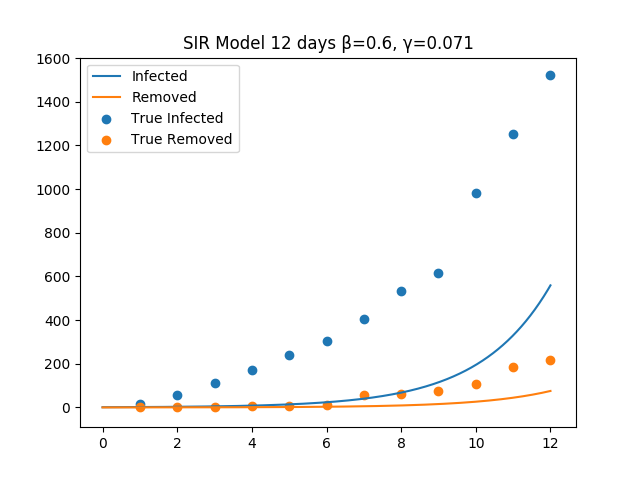
\includegraphics[scale=0.5]{../Fig1.png}
	\\
	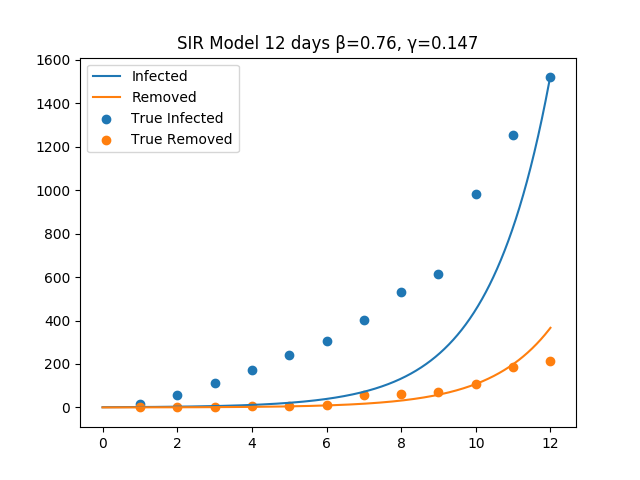
\includegraphics[scale=.5]{../Fig2.png}
	\caption{The figures above show the how the SIR model changes after the optimal $\beta$ is computed.}
\end{figure}
\section{Results}
Once we run the simulation for the SIR modeling over a full period of 120 days we find out that the peak in infection will be reached between the 27th and the 31st day of the infection. Furthermore the critical proportion of the people to be vaccinated, to gain hard immunity, in case a vaccine is developed need to be around the $80\%$ of the population. This model did not take into consideration the measure that were adopted by the Government after the 1st of March to control the spread of COVID-19.
\begin{figure}[h]
	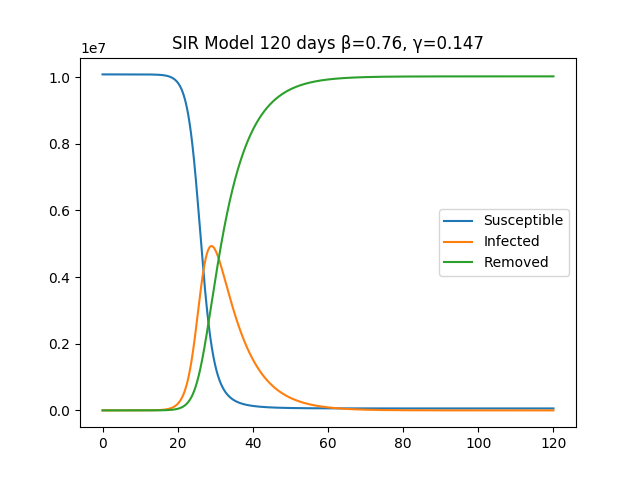
\includegraphics[scale=.5]{../Fig3.png}
	\caption{The figures above show the simulation for the above described SIR model over the duration of 120 days.}
\end{figure}
\bibliographystyle{unsrt}
\bibliography{main}
\end{document}
